%
\documentclass[10pt,a4paper]{article}


\usepackage{array}
\usepackage{subfigure}
\usepackage{graphicx}
\usepackage{amssymb}
\usepackage{amsmath}
\usepackage{cite}
\usepackage{color}
\usepackage{url}
\usepackage[lined,linesnumbered,ruled,norelsize]{algorithm2e}
\usepackage{listings}
\lstset{
  language=Octave, 
  basicstyle=\footnotesize, 
  frame=single, 
  showspaces=false, 
  showstringspaces=false}




\begin{document}

\title{Experiment 7: Non-linear SVM Classification With Kernels}

\maketitle
  
\section{Description}
%
  In this exercise, you will an RBF kernel to classify data that is not linearly separable. As in the last exercise, you will use the LIBSVM interface to MATLAB/Octave to build an SVM model. If you do not already have LIBSVM on your computer, refer to the previous exercise for directions on installing and running LIBSVM.

  To begin, download and unzip the data for this exercise: ex7Data.zip.
  


\section{Kernel}
%
  Recall from the lecture videos that linearly non-separable features often become linearly separable after they are mapped to a high dimensional feature space. However, we don't ever need to compute the feature mappings $\phi(x^{(i)})$ explicitly: we only need to work with their kernels, which are easier to compute. Therefore, it's possible to create a very complex decision boundary based on a high dimensional (even infinite dimensional) feature mapping but still have an efficient computation because of the kernel representation.

  In this exercise, you will use the Radial Basis Function (RBF) kernel in LIBSVM. This kernel has the formula
  %
  \begin{figure}[htb!]
    \centering
      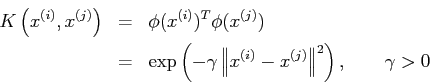
\includegraphics[width=.7\columnwidth]{img81}
  \end{figure}
  %
  
  Notice that this is the same as the Gaussian kernel in the video lectures, except that term  $\frac{1}{2\sigma^2}$ in the Gaussian kernel has been replaced by $\gamma$. Once again, remember that at no point will you need to calculate $\phi(x)$ directly. In fact, $\phi(x)$ is infinite dimensional for this kernel, so storing it in memory would be impossible.




\section{Example 1}
%
  Now let's see how an RBF kernel can choose a non-linear decision boundary. Load the LIBSVM-formatted data ``ex7a.txt'' into your Matlab/Octave workspace using the command
  %
  \begin{lstlisting}
    [train_labels, train_features] = libsvmread('ex7a.txt');
  \end{lstlisting}

  This is a two-dimensional classification problem, and if you plot the positives and negatives using different colors, you should get an image like the one below.
  %
  %
  \begin{figure}[htb!]
    \centering
      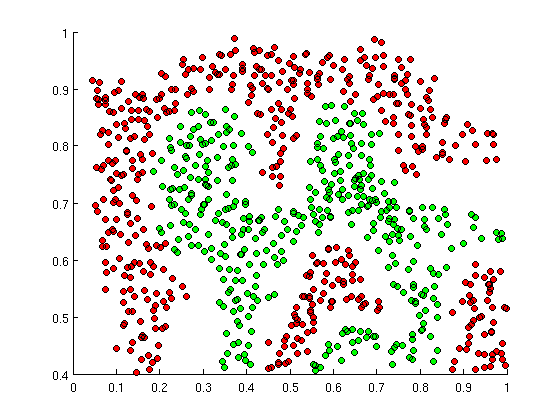
\includegraphics[width=.7\columnwidth]{ex8a_dataonly}
  \end{figure}
  %
  There's no linear decision boundary for this dataset, but we'll see now how an RBF kernel can automatically decide a non-linear one.

  Using the svmtrain command that you learned in the last exercise, train an SVM model on an RBF kernel with $\gamma = 100$. If you don't remember how to set the parameters for this command, type ``svmtrain'' at the MATLAB/Octave console for usage directions.

  Once you have the model, you can use the ``plotboundary'' command that we have provided to visualize the decision boundary.
  %
  \begin{lstlisting}
    plotboundary(train_labels, train_features, model);
  \end{lstlisting}
  %
  This gives you the following result:
  %
  %
  \begin{figure}[htb!]
    \centering
      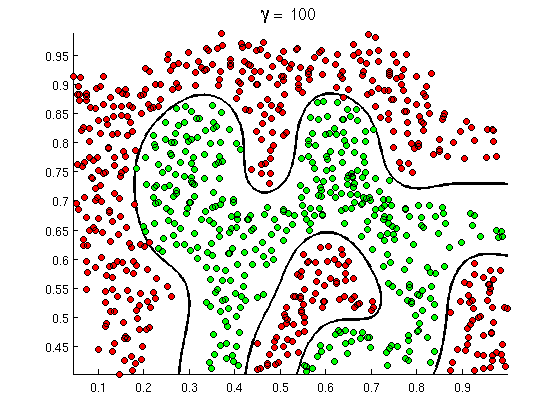
\includegraphics[width=.7\columnwidth]{ex8a_nofill}
  \end{figure}
  %
  The plotboundary command includes an option for seeing the filled-in contours of the  $\sum_i \alpha_i K(x^{(i)}, x) + b$ function. Remember that this function gives the decision values that are used to make a classification. An example  $x$ is classified as a positive example if  $\sum_i \alpha_i K(x^{(i)}, x) + b \geq 0$, and is classified negative otherwise.

  To activate this option, type
  %
  \begin{lstlisting}
    plotboundary(train_labels, train_features, model, 't');
  \end{lstlisting}
  %
  The result will look like the image below.
  %
  %
  \begin{figure}[htb!]
    \centering
      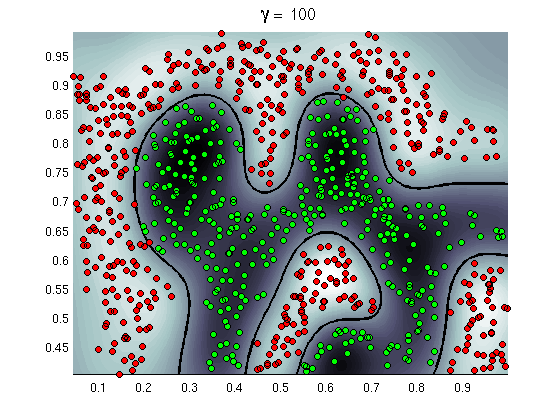
\includegraphics[width=.7\columnwidth]{ex8a_fill}
  \end{figure}
  %
  Intuitively, you can think of the white areas as the highest-confidence regions for positive classification, and the black areas as the highest-confidence regions for negative classification. The color gradient shows the change in decision values for making classifications.


\section{Example 2}
%
  In this second example, we'll look at how the parameter  $\gamma$ in the RBF kernel affects the decision boundary.

  Load the data file ``ex7b.txt'' into your workspace and plot the data. Your result should look similar to this:
  %
  \begin{figure}[htb!]
    \centering
      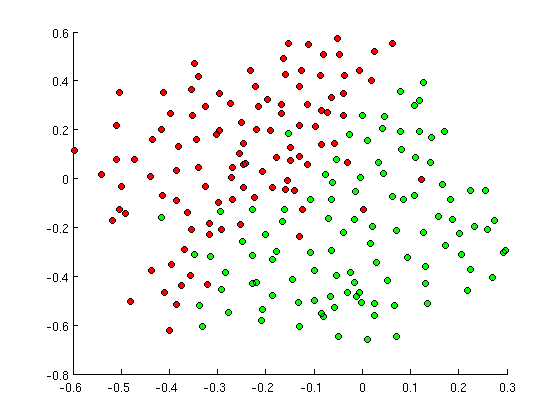
\includegraphics[width=.7\columnwidth]{ex8b_dataonly}
  \end{figure}
  %
  Now train your model using $\gamma$ values of 1, 10, 100, and 1000 and plot the decision boundary (using no contour fill) for each model. How does the fit of the boundary change with $\gamma$?






\end{document}